\subsection{Spark it up}
Før vi kan begynne å lage aggregeringer, må vi gjøre datasettene om til Parquet filer. Det er alltid lurt å gjøre om til Parquet først, siden de tilbyr komprimering.

\subsubsection{Generell kode for lesing/skriving}
\code{Scala}{code/milepael5/code.scala}

\subsubsection{Student Performance Dataset (KV-database)}
% Aggregering 1 %
\textbf{Første Aggregering}\\
\code{Scala}{code/milepael5/agg1.scala}

% Aggregering 2 %
\textbf{Andre Aggregering}\\
\code{Scala}{code/milepael5/agg2.scala}

% Aggregering 3 %
\textbf{Tredje Aggregering}\\
\code{Scala}{code/milepael5/agg3.scala}

\subsubsection{Socio-Economic Country Profiles (Dokumentdatabase)}
% Aggregering 1 %
\textbf{Første Aggregering}\\
\code{Scala}{code/milepael5/countryFirst.scala}

% Aggregering 2 %
\textbf{Andre Aggregering}\\
\code{Scala}{code/milepael5/countrySec.scala}

\subsubsection{World University Rankings (Kolonnefamiliedatabase)}

Først leser vi csv filen med "inferSchema" satt til "true" for å opprette schema.

Jeg legger merke til at noen av datatypene ikke stemmer. Jeg ser at "world rank" er satt til streng, selv om det tilsynelatende er int. Men det går fin, siden den også inneholder verdier som "100 150". Derimot, "international" var satt til streng, fordi null-verdier var byttet ut med bindestrek , I tillegg så jeg at "international students" hadde verdier med tall og prosent-tegnet. Begge fikset jeg ved å bruke find and replace funksjonen i libreOffice og endre på csv-filen.

Da brukte jeg universityDf.printSchema() igjen for å sjekke at ting stemte, og det gjorde det.
\FigureCounter
\begin{figure}[H]
    
\includegraphics[width=\textwidth]{images/milepael5/printSchema.png}
\end{figure}

Det neste er å lagre den som en Parquet fil.

\code{Scala}{code/milepael5/readUniversitySaveToParquet.scala}

% Aggregering 1 %
\textbf{Første Aggregering}\\
Den første aggregeringen jeg lagde viser de ti skolene med flest kvinnelige studenter. 

\code{Scala}{code/milepael5/universityByFemaleRatio.scala}
\FigureCounter
\begin{figure}[H]
    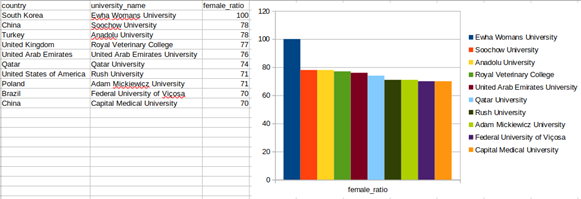
\includegraphics[width=\textwidth]{images/milepael5/resUniFemRatio.png}
\end{figure}

% Aggregering 2 %
\textbf{Andre Aggregering}\\
Denne er tilsvarende forrige aggregering, men denne gangen for mannlige studenter.

\code{Scala}{code/milepael5/universityByMaleRatio.scala}
\FigureCounter
\begin{figure}[H]
    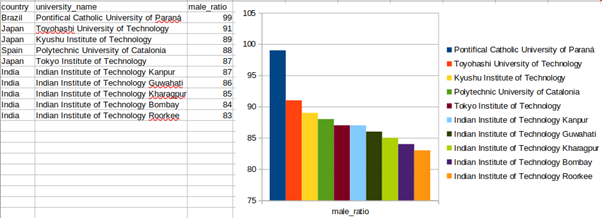
\includegraphics[width=\textwidth]{images/milepael5/resUniMaleRatio.png}
\end{figure}

% Aggregering 3 %
\textbf{Tredje Aggregering}\\
Jeg lagde også en aggregering som viser gjennomsnitts-poeng per år. Denne var, til å begynne med, ment til å representere "Average Total Score by Number Of Students" komponentet fra forrige milepæl:

\FigureCounter
\begin{figure}[H]
    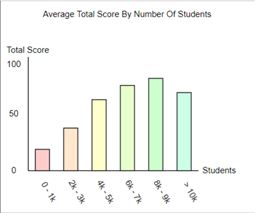
\includegraphics[width=\textwidth]{images/milepael5/avgScoreTotStudents.png}
\end{figure}

Her er den nye aggregeringen:

\FigureCounter
\begin{figure}[H]
    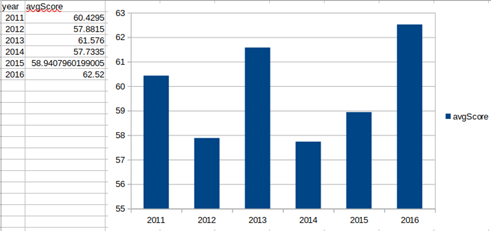
\includegraphics[width=\textwidth]{images/milepael5/avgScoreTotStudentsActual.png}
\end{figure}

\subsubsection{Government Types Of The World (Grafdatabase)}
Begynner med å lese csv filene. Merk at i dette datasettet er det 4 forskjellige csv-filer. Så skrive de til parquet filer.

\code{Scala}{code/milepael5/readWriteREIGN.scala}
% Aggregering 1 %
\textbf{Første Aggregering}\\
Her lagde jeg kun en aggregering, men til prosjektinnleveringen vil vi bruke de andre også. Aggregeringen viser hvordan hver styremåte har utviklet seg i popularitet gjennom årene. Den opprinnelige skissen fra milepæl 4 ser slik ut:

\FigureCounter
\begin{figure}[H]
    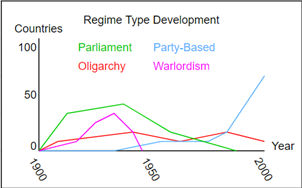
\includegraphics[scale=1.0]{images/milepael5/regimeTypeGraphic.png}
\end{figure}

Til å begynne med, tenkte jeg å gruppere først på år, så på styremåte, og dermed telle antall opplistinger.

\code{Scala}{code/milepael5/governmentPopularityFirst.scala}

Men dessverre var ikke dette optimalt for lesing av grafiske programmer (excel, libreoffice). Så jeg bestemte meg for å gjøre om på komponenten. I denne nye versjonen har jeg en kolonne for år, og en kolonne for hver styremåte. Da ble aggregeringen slik:

\code{Scala}{code/milepael5/governmentPopularityByYear.scala}

Framstilling i libreoffice:

\FigureCounter
\begin{figure}[H]
    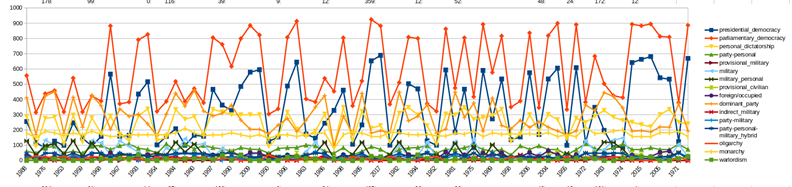
\includegraphics[width=\textwidth]{images/milepael5/libreOfficeGovPop.png}
\end{figure}

\subsubsection{Endringer på nettsiden}
Vi fant ut i denne milepælen at dynamisk brukerinput ville være vanskelig å inkorporere i noen av aggregeringene, som f.eks land-aggregeringene i dokumentdatabasene. Derfor ville det vært vesentlig mindre brukerinteraksjon på nettsiden.